% Experimental method

The following section presents an overview of autoencoder network architectures and estimation methodology employed to evaluate the role of compression and bias hyperparameters in reconstruction accuracy of encoded images. 
To this end, the analysis in this note adopts a fundamentally simple experimental framework, whereby a generic autoencoder architecture is iteratively modified and reviewed for changes in reconstruction performance.
This generic architecture (illustrated in Figures \ref{fig:autoencoder-diagram} and \ref{fig:autoencoder-diagram-bias}) consists of an input layer with 784 nodes; a single fully-connected hidden layer with a variable number of nodes activated by the Sigmoid function; an optional bias node; and an output layer with 784 nodes---again, activated by the Sigmoid function.

To assess the role of compression ratios in reconstruction performance, the generic autoencoder architecture is sequentially modified by varrying number of nodes in the hidden layer across seven values: 2, 4, 8, 14, 28, 56, and 112.
This generates seven distinct autoencoder architectures, with corresponding compression ratios of 392x, 196x, 98x, 56x, 28x, 14x, and 7x respectively.
Each architecture is modelled twice: once with the inclusion of trainable bias weights, and once with bias weights set to zero.
Figures \ref{fig:autoencoder-diagram} and \ref{fig:autoencoder-diagram-bias} present diagrams of the generic autoencoder architecture with and without trainable bias weights. 

In total, the employed experimental framework estimates fourteen distinct combinations of autoencoder architectures, spanning across seven parameterisations of compression ratios, and two parameterisations of bias nodes. 
Each model is trained on a training partition of the MNIST dataset (N=60,000) for 50 epochs.
Learning rate is set at 0.01, and invariant between models.
At the end of each epoch, reconstruction accuracy of each autoencoder is assessed by calculating mean squared error (MSE) across the validation partition of the training dataset (N=10,000).
Traces of MSE for each model architecture throughout the training phase are presented in Figure \ref{fig:training-loss}.


\begin{figure}
    \caption{Generic autoencoder architecture, without bias}
	\label{fig:autoencoder-diagram}
	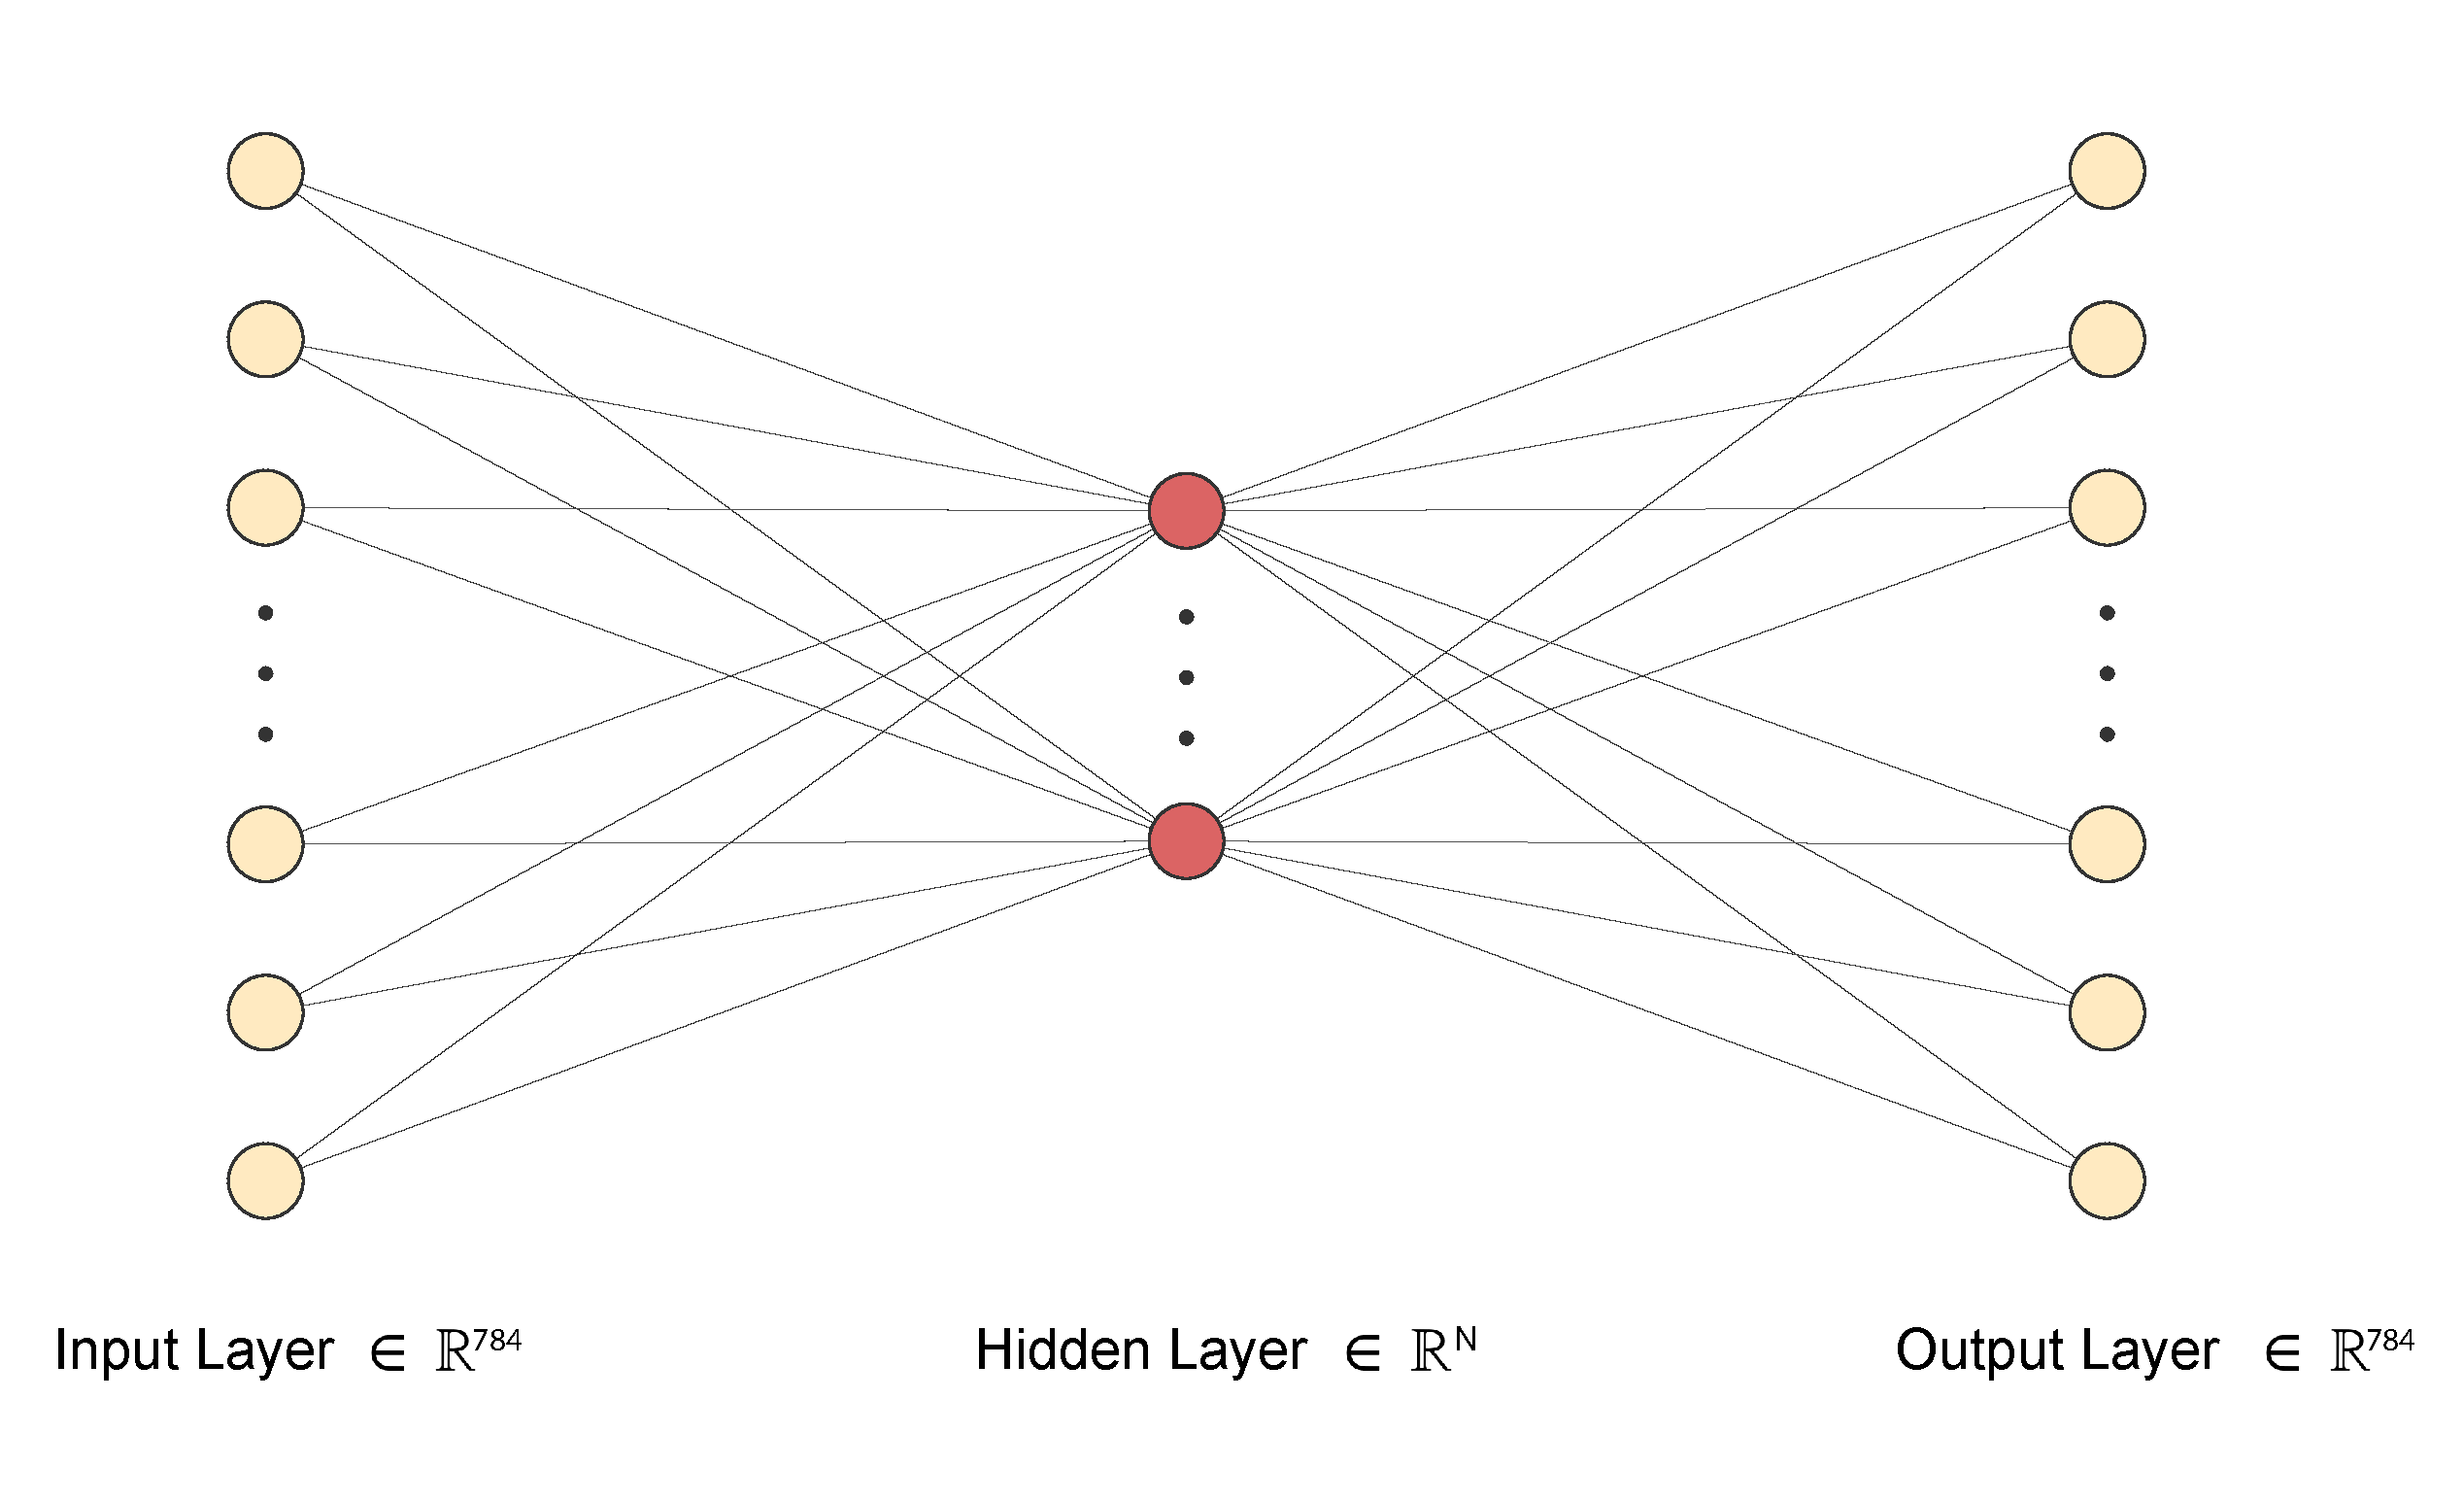
\includegraphics[width=1.0\textwidth]{graphics/autoencoder_diagram.pdf}
    \textbf{Notes}: Input and output layers each contain 784 nodes respectively, in congruence with the dimensions of MNIST image instance vectors. Intermediate nodes are omitted for ease of interpretability. Hidden layers contain a variable number of nodes, $N$, varied across seven values: 2, 4, 8, 14, 28, 56, and 112. Encoding of inputs occurs through weighting of activations between input and hidden layers. Image reconstruction occurs through weighting of activations between hidden and output layers.
\end{figure}

\begin{figure}
    \caption{Generic autoencoder architecture, with bias}
	\label{fig:autoencoder-diagram-bias}
	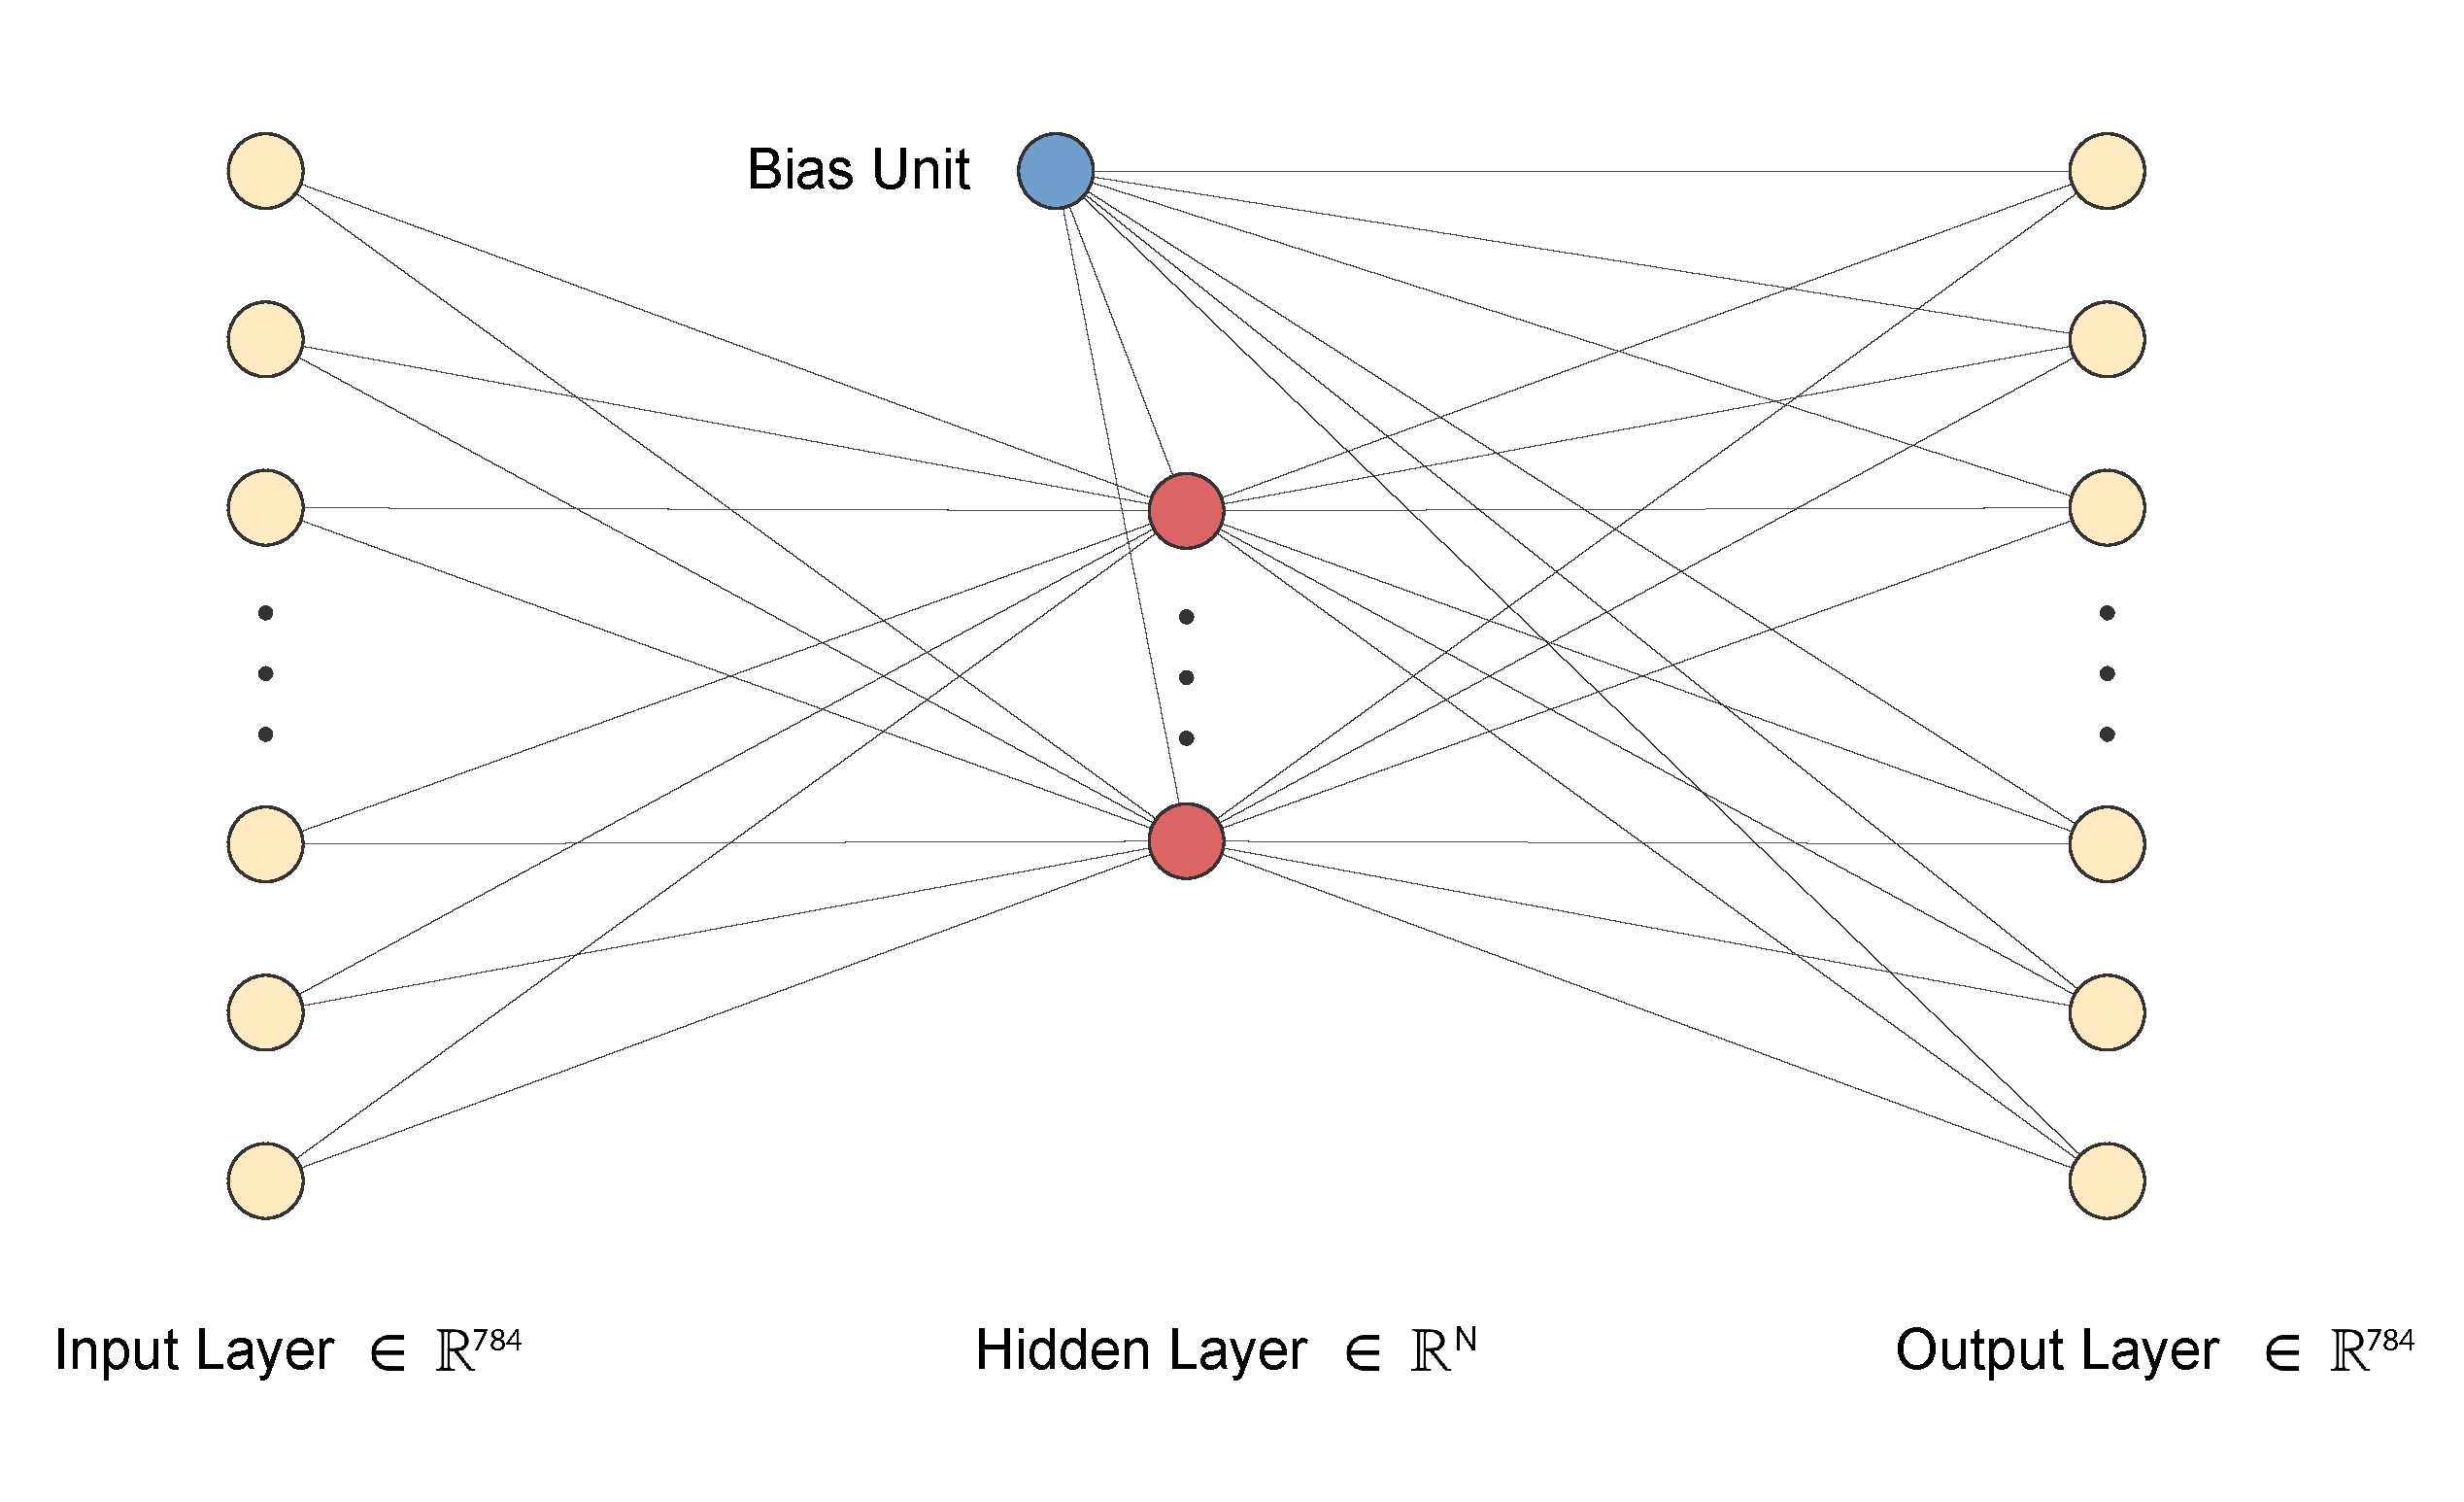
\includegraphics[width=1.0\textwidth]{graphics/autoencoder_diagram_bias.pdf}
    \textbf{Notes}: Input and output layers each contain 784 nodes respectively, in congruence with the dimensions of MNIST image instance vectors. Intermediate nodes are omitted for ease of interpretability. Hidden layers contain a variable number of nodes, $N$, varied across seven values: 2, 4, 8, 14, 28, 56, and 112. A  constant bias affects activations in hidden and output nodes differentially through learned bias weights. Encoding of inputs occurs through weighting of activations between input and hidden layers. Image reconstruction occurs through weighting of activations between hidden and output layers. 
\end{figure}

\begin{figure}
    \caption{Reconstruction mean-squared error throughout training phase, disaggregated by network architecture}
	\label{fig:training-loss}
	\includegraphics[width=1.0\textwidth]{graphics/model_loss.pdf}
    \textbf{Notes}: Mean-squared error (MSE) of autoencoder networks across validation partition of MNIST dataset. MSE was calculated through forward propogation of MNIST validation instances (N=10,000) using trained weights at each discrete training timestep. Learning rate for each model was set at 0.01.
\end{figure}